% \documentclass[conference]{IEEEtran}
\documentclass[conference,compsoc]{IEEEtran}
% \documentclass[journal]{IEEEtran}
% \documentclass[10pt,journal,compsoc]{IEEEtran}
% \documentclass[journal,comsoc]{IEEEtran}
% \documentclass[journal,transmag]{IEEEtran}

\usepackage[utf8]{inputenc}
\usepackage[T1]{fontenc}

% \usepackage[ngerman]{babel}
\usepackage{ifpdf}
\usepackage[numbers]{natbib}
\usepackage{graphicx}
\usepackage{multirow}
\usepackage{amsmath}
\usepackage{algorithmic}
\usepackage{array}

% IEEEtran contains the IEEEeqnarray family of commands that can be used to
% generate multiline equations as well as matrices, tables, etc., of high
% quality.

\ifCLASSOPTIONcompsoc
  \usepackage[caption=false,font=footnotesize,labelfont=sf,textfont=sf]{subfig}
\else
  \usepackage[caption=false,font=footnotesize]{subfig}
\fi

\usepackage{float}
\usepackage{stfloats}
\usepackage{url}


\hyphenation{}

\begin{document}
\title{A review of the rkmh toolkit and its possible applications}

\author{
  \IEEEauthorblockN{Christoph Stach}
  \IEEEauthorblockA{
    Hochschule für Technik und Wirtschaft Berlin\\
    Fachbereich 4 - Angewandte Informatik\\
    s0555912@htw-berlin.de
  }
}

\maketitle

\begin{abstract}
The rkmh toolkit is a collection of algorithms and filtering methods recently released. It is used for the classification of reads of DNA sequencing technologies. The authors of the algorithm state, that it is especially useful and more for finding co-infections of different but similar sublineages of viruses. They demonstrate their results for the Human papillomavirus (HPV) by presenting different statistics of their algorithm. Rkmh is based on a technique called MinHashing, which used in the field of text mining. This work aims to supplement the original paper of the rkmh toolkit by drawing a connection between the field of text mining and bio informatics. Also the author compares it to other algorithm and gives a brief perspective about alternative use cases.
\end{abstract}
  
\section{Introduction}

Mauris elit elit, mattis ut.\\





\section{Fundamentals}

In the section fundamentals for understanding the rkmh toolkit are explained. The autor gives a brief explanation with example for the jaccard coefficient, hash functions in general and the MinHash algorithm.

\subsection{Jaccard coefficient}

The Jaccard coefficient is a metric used to measure the similarity of two sets.\\

\begin{equation}
    J(A,B) = \frac{ | A \cap B | }{ | A \cup B | }
\end{equation}\\

It is calculated by counting the intersection of $ A $ and $ B $ and dividing it by the count of union of $ A $ and $ B $. The result is a rational number between $ 0 $ and $ 1 $, where numbers close to $ 1 $ mean that the compared sets are similar. Having two sets which are completely equal generate a jaccard coefficient of $ 1 $.\\

\begin{figure}[H]
    \centering
    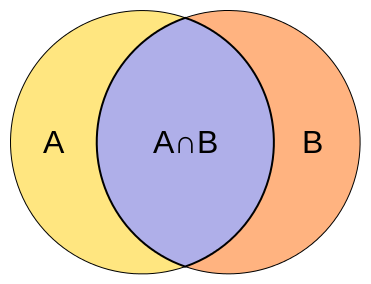
\includegraphics[width=0.20\textwidth]{images/Intersection_of_sets_A_and_B.png} 
    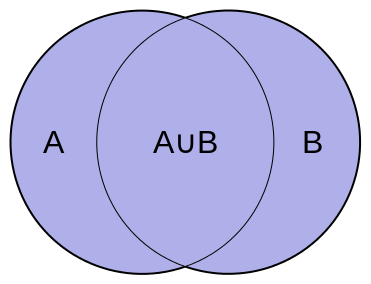
\includegraphics[width=0.20\textwidth]{images/Union_of_sets_A_and_B.png}
    \caption{Intersection and union of two sets $ A $ and $ B $ \cite{intersectionImage,unionImage}}
\end{figure}

Calculating the Jaccard coefficient for two sets and a total of $ n $ items has a complexity of $ O(n^2) $. For high dimensional sets, sets that contain a lot of items, which have therefor a large $ n $, the curse of dimensionality applies very quickly.\\
\subsection{Hash functions}
A hash function $ h $ is a usually quickly to compute function which takes  items of any set $ S $ and maps it to a fixed size number $ n $. Therefore it generates a signature for the items. The signatures upper bound is fixed by $ n $. Having enough items in $ S $, it can happen that different items are assigned the same signature and are not distinguishable any more. This is called a collision.\\

\begin{table}[h!]
    \centering
    \begin{tabular}{| c | c | c | c | c | c |}
        \hline
        0  & 1  & 2  & 3  & 4  & 5  \\
        \hline
           & 30 &    & 10 &    & 11 \\
        \hline
           &    &    &    &    & 41 \\
        \hline
    \end{tabular}   
\end{table}
    
In the example above the hash function $ h(x) = (2x+1) \mod 6 $ assigns signatures to the elements of set $ S = \{ 10,11,30,41 \} $.  In this case $ n $ is $ 6 $ and the numbers $ 11 $ and $ 41 $ get the same signature assigned, which leads to a collision.\\

Hash functions exist for different purposes. There are many used in the field cryptographics \cite{cryptographicHashFunctions}, which try to avoid collisions. But also non-cryptographic hash function are available, which do not share this property. The second kind of hash function is used in dimensionality reduction and similarity estimation of datasets \cite{practicalHashFunctions}.\\
\subsection{MinHash}
\label{ssec:minhash}

MinHashing is a often used technique to compare big datasets. I is used in data-mining and was first applied by \citeauthor{minhash} to compare a large corpus of crawled web pages \cite{minhash}. It works by reducing the dimensionality of sequences (also often called documents). The algorithm assigns a signature to a document. These signature signatures have the property to reflect the similarity of the documents. \\

\subsubsection{Shingling}

Given two documents $ A = "abccdab" $ and $ B = "bccdacb" $. The documents are first converted into a sets of shingles with the size of $ k $. For $ k = 3 $ the resulting sets are: \\

\begin{equation}
    \begin{split}
        S_k(A) = \{abc, bcc, ccd, cda, dab\} \\
        S_k(B) = \{bcc, ccd, cda, dac, acb\} \\
        S_k(A) \cup S_k(B) = \{abc, bcc, ccd, cda, dab, dac, acb\}
    \end{split}
\end{equation}\\

Documents and shingles can now be represented as a sparse matrix, where the shingles are the rows and the documents the columns. The computed Jaccard coeeficcient of A and B is  $ J(S_k(A),S_k(B)) = \frac{3}{7} \approx 0.43 $.\\

\subsubsection{Matrix representation}

For the purpose of this algorithm we build a sparse matrix of all shingles of the union of $ S_k(A) $ and $ S_k(B) $. Instead of writing the shingles directly to the matrix, we write a $ 1 $ if the shingle occurs in the document otherwise we write a $ 0 $. With the data from the previuose this leads to a the matrix representation $ M $. The columns represent a document and the rows the shingles. \\

\begin{equation}
    \begin{split}
        P = 
        \begin{pmatrix}
            0 & 3 & 5 & 4 \\
            1 & 6 & 4 & 1 \\
            2 & 2 & 1 & 2 \\
            3 & 5 & 3 & 6 \\
            4 & 1 & 2 & 3 \\
            5 & 0 & 0 & 5 \\
            6 & 4 & 6 & 0
        \end{pmatrix}
        M = 
        \begin{pmatrix}
            1 & 0 \\
            1 & 1 \\
            1 & 1 \\
            1 & 1 \\
            1 & 0 \\
            0 & 1 \\
            0 & 1
        \end{pmatrix}   
    \end{split}
\end{equation} \\

Also we store a matrix $ P $ of random permutations of the row indecies. We use them to generate the signature for the columns on the next step\\  



\subsubsection{Generation of a signature}





% Hier weitermachen
\section{Rkmh}

The rkmh toolkit uses the MinHash algorithm to convert reads (documents in context of text mining) to sketches (signatures in context of text mining). It first uses MurmurHash3, non-cryptographic hash function, to convert k-mers (k-shingles / k-grams in the context of text mining) to 64bit integer values. Before generating the sketch-signature, rkmh uses different kind of filters to the reduce the number of hashes the sketch is calculated of.\\

Rkmh offers different filters. It can remove hashes that total number of occurrences doesn't meet a defined threshold. Seldom occurring hashes are prone to be sequencing errors. Also k-mers that occur to many times can be filtered, because they are shared by many DNA sequences and are not informative for classifying.\\

More filters are available and are described in the original paper \cite{rkmh}. By providing the different filters the number of hashes the sketch is calculated of can be reduced by a great amount. This has positive impact on the performance of the toolkit. The authors state that classification can be done within minutes on a standard laptop.
\section{Comparison with other algorithms}


BLAST (Basic Local Alignment Search Tool) \cite{blast} finds regions of similarity between biological sequences. It was developed in 1990 and databases of biological sequences were much smaller in this time period. Today new sequencing technologies produce much more data. Today, researches are striving to develop new tools to handle this increase.\\

Mash \cite{mash} uses MinHashing to reduce large biological sequences to small sketches. By comparing sketches pairwise, mutation distances between sequences can be estimated. This enables clustering and searching a huge sequences sets.\\

Rkmh builds up on the on mash \cite{mash}. It uses MinHashing and extends Mash by adding different filters.\\

Sourmash \cite{sourmash} also uses MinHashing. It is designed to facilitate containment and similarity queries for taxonomic exploration within large datasets.\\

\section{Alternative use cases}

MinHashing has a lot of application in text mining. It can be used to make large collection of documents searchable and comparable. The MinHash is calculated for each document and then compared to the MinHash of a search query.\\

Another possible application is a toolkit for checking for plagiarism of scientific documents. Given a large database of documents, the MinHash is calculated and stored for each document. After calculating the MinHash for a newly submitted document, it can be compared to all documents in the database. A similarity threshold determines if the document is a plagiarism or not. Further, similar documents can be shown for a manual review. Filtering options, like in rkmh, can reduce the total number of shingles and improve the results and performance of the toolkit.\\

Finally music songs can be compared with MinHashing. Music songs are sequences of notes. Therefore, they can be shingled. The application would work similarly to the plagiarism toolkit or rkmh. A MinHash for each song is calculated and stored along with a song in a database. An application could record the sounds in the direct environment of a microphone and compare it to the songs stored in the database to find a song the user is currently listening to.\\
\section{Conclusion}

In this work the author explained the functionality of MinHashing. The technique originally came from the field of text mining and is now used in various applications of bio informatics \cite{rkmh, mash, sourmash}.\\

The focus lied on the rkmh toolkit, wich uses MinHashing for classification of infections and co-infections of various viruses.\\

It is clear to say that MinHashing is well suited for comparison and similarity estimation of large sets of DNA sequences. Therefor it is an interesting topic in the field of bio informatics.\\

\newpage

\bibliographystyle{IEEEtranN}
\bibliography{IEEEabrv,references/scientific}

\end{document}